\section{Техническое задание}

В курсовой работе необходимо выполнить следующие пункты:

\begin{enumerate}[label*=\arabic*.]

\item Анализ цепи во временной области. 

Анализу подлежит цепь, схема которых задана в табл. \ref{tab:circ}
тройками чисел \cite{tasks} в соответствии с номером варианта задания.
Независимые начальные условия нулевые. 
В момент времени $ t = 0 $ на вход цепи подан сигнал 
в виде ступенчатой функции 
напряжения $ U_1 \delta_1 (t) $ или
тока $ I_1 \delta_1 (t) $
где $ U_1 = 1В $; $ I_1 = 1А $. 
Фактически нормированные параметры $ R-, L-, C- $элементов 
заданы соответственно в омах, генри, фарадах. 
Требуется:

\begin{enumerate}[label*=\arabic*.]
    \item Составить уравнения состояния цепи для $ t \ge 0 $.
    \item По уравнениям состояния аналитическим расчетом во временной
    области найти переходную характеристику $ h_1(t) $
    для реакции и построить ее график. 
    В предлагаемых цепях реакцией (т. е. выходным сигналом) является
    напряжение нагрузки $ u_2(t) $ или ток нагрузки $ i_2(t) $.
\end{enumerate}

\begin{table}[H]
    \centering
    \begin{tabular}{|c|p{10cm}|}
        \hline
        Вариант & Цепь \\
        \hline
        11 & 114 -- ИН $ u_1 $;
        224 -- $ R_н = 1 $;
        313 -- $ R_3 = 2 $;
        434 -- $ R_4 = 2 $;
        513 -- $ L_5 = 0.5 $;
        632 -- $ L_6 = 1 $; \\
        \hline
    \end{tabular}
    \caption{Цепь}
    \label{tab:circ}
\end{table}

\item Анализ цепи операторным методом 
при действии одиночного импульса на входе.

В момент времени $ t = 0 $ на вход цепи, 
заданной в п. 1, при нулевых независимых начальных условиях 
подается сигнал в виде одиночного импульса
напряжения или тока, форма которого 
приведена на рис. \ref{fig:task_plot}.
Параметры сигнала:

\begin{equation}\label{eq:params}
\begin{cases}
    U_m = 7 В\\
    t_и = 3.0 с\\
    T = 9 с\\
\end{cases}
\end{equation}

Требуется:

\begin{enumerate}[label*=\arabic*.]
    \item В соответствии с номером выполняемого варианта определить
    функцию передачи напряжений $ H_U(s) $ или токов $ H_I(s) $.
    Осуществить проверку функции передачи при 
    $ s = 0 $ и $ s \rightarrow \infty $; 
    представить соответствующие этим значениям схемы замещения цепи.
    \item Найти нули и полюсы функции передачи
    и показать их расположение на плоскости комплексной частоты. 
    По значениям полюсов функции передачи 
    дать заключение о характере и практической 
    длительности переходного процесса.
    \item Определить переходную $ h_1(t) $ характеристику цепи, 
    сравнить с найденной в п. 1.2 задания. 
    Проверить $ h_1(0) $ и $ h_1(\inf) $ 
    по аналитическому выражению $ h_1(t) $ и непосредственно по схеме цепи.
    \item Определить изображение по Лапласу входного одиночного импульса.
    \item Определить изображение выходного сигнала и далее
    найти реакцию $ i_2(t) $ или $ u_2(t) $ во временной области.
    Построить графики входного и выходного сигналов на одном рисунке.
\end{enumerate}

\begin{figure}[H]
    \centering
    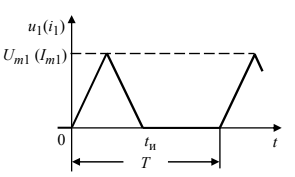
\includegraphics[width=0.7\linewidth]{photo/task_plot}
    \caption{Форма входного сигнала}
    \label{fig:task_plot}
\end{figure}

\item Анализ цепи частотным методом 
при действии одиночного импульса на входе.

Условия заданы в п. 2 задания. 
Требуется:

\begin{enumerate}[label*=\arabic*.]
    \item Используя найденное в 2.1 выражение 
    $ H_U(s) $ или $ H_I(s) $, 
    вычислить и построить графики АЧХ и ФЧХ функций передачи цепи 
    $ H_U(j\omega) $ или $ H_I(j\omega) $.
    Произвести проверку АЧХ при $ \omega = 0 $ и $ \omega \rightarrow \infty $.
    \item Определить полосу пропускания цепи по уровню 
    $ 0.707|H(j\omega)|_{max} $.
\end{enumerate}

\end{enumerate}